\graphicspath{{experimental_setup/fig/}}

\chapter{Experimental Setup} \label{chap:experimental_setup}
This chapter provides our research question, and how we attempt to answer
this question using the results of different experiments. We discuss the speech data used for
our ASR models, as well as the text data used for our language model (LM).
The chapter ends with a discussion of the metric used to evaluate our ASR models.

% FIX FIX FIX
\section{Research question and experiments}
The focus of our research is performing ASR for Afrikaans and isiXhosa with limited speech data and computational resources.
Our main research question is determining whether the use of additional Dutch and isiZulu speech data can help develop ASR systems for Afrikaans and isiXhosa.

Our approach involves fine-tuning (\ref{subsec:finetune}) the \href{https://huggingface.co/facebook/wav2vec2-xls-r-300m}{XLS-R (300M)} model using different training strategies.
Two training strategies are considered in this study. 
The first strategy is called \emph{basic fine-tuning} and it involves fine-tuning XLS-R (300M) on one dataset (one language). 
The second strategy is called \emph{sequential fine-tuning} and it involves fine-tuning XLS-R (300M) on two datasets (two languages) separately. 
The intent of sequential fine-tuning is to first fine-tune on the related language (e.g. Dutch) and then fine-tune on the target language (e.g. Afrikaans).
We create several models using both training strategies, and each model is evaluated using the word error rate (WER) (\ref{subsec:wer}).
We choose the best Afrikaans and isiXhosa model for both strategies based on which model has the lowest WER on our validation data.
Finally, we add a $5$-gram LM (\ref{subsec:lm-boost}) to our best-performing models (to improve performance) and evaluate the models on our test data.

The following hyperparameters are tuned during the training of each model: 
\texttt{batch size}, \texttt{gradient accumulation steps}, \texttt{evaluation steps}, and \texttt{patience}.
To clarify, \texttt{evaluation steps} refers to the number of steps between each evaluation on the validation data,
and \texttt{patience} refers to the hyperparameter used for early stopping \cite{wikipedia2023early_stopping}. 
We use early stopping on the validation data to prevent our models from overfitting on the training data.

\section{Data}\label{sec:data}
We use three different speech datasets
to create an \href{https://huggingface.co/datasets/lucas-meyer/asr_af}{Afrikaans dataset} 
and an \href{https://huggingface.co/datasets/lucas-meyer/asr_xh}{isiXhosa dataset}, which contains transcribed speech data.
We also use one of the datasets to create Dutch and isiZulu datasets.
We discuss the three datasets in the paragraphs below.

\paragraph*{NCHLT.}
The NCHLT \cite{barnard2014nchlt} dataset contains transcribed speech data for the eleven official South African languages.
The dataset contains approximately $200$ speakers per language.
The NCHLT recordings (on average) are the shortest of the three datasets, with most recordings being between $2$ and $6$ seconds.
Based on a brief inspection, the transcription texts of this dataset contain very few words and rarely contain full sentences.

\paragraph*{FLEURS.}
The FLEURS \cite{fleurs2022arxiv} dataset contains transcribed speech data for $102$ different languages, including Afrikaans, Dutch, isiXhosa, and isiZulu.
Each language has its own training, validation, and test data split.
No information is given about the number of speakers for each language.
The FLEURS recordings (on average) are the longest of the three datasets, with most recordings being between $7$ and $20$ seconds.
Based on a brief inspection, the transcription texts of this dataset contain full sentences.

\paragraph*{High-quality TTS.}
The High-quality text-to-speech (TTS) \cite{hq2017} dataset contains high-quality transcribed speech data for four South African languages: Afrikaans, Sesotho, Setswana and isiXhosa.
There are nine Afrikaans speakers and 12 isiXhosa speakers.
The duration of most recordings is between $5$ and $10$ seconds.
Based on a brief inspection, the transcription texts of this dataset contain mostly full sentences and a few that contain short phrases.
\\
\\
As mentioned, we select recordings from the three datasets to create the final Afrikaans and isiXhosa datasets.
Additionally, we use the Dutch and isiZulu data from the FLEURS dataset for our sequential fine-tuning experiments.

\subsection{Approach for selecting recordings}
To optimize training and GPU memory usage, we select recordings to maintain a roughly uniform distribution in terms of their durations.
This approach mitigates the challenges of random batch selection during fine-tuning.
Since batches are selected randomly, one batch may contain much longer recordings than another batch.
Inconsistent batch durations may lead to suboptimal GPU memory allocation, leading to all of the GPU memory being used and triggering an exception.
The NCHLT dataset contains much more data than the other two datasets. However, the NCHLT recordings are much shorter and of lower quality. 
Consequently, we omit a large portion of the NCHLT dataset in favor of the recordings from the other two datasets.
Figure \ref{fig:histogram1} describes the histograms of the recording durations of the two datasets without removing outliers,
Figure \ref{fig:histogram2} describes the histograms of the recording durations of the two datasets after removing outliers.
Note that we lose a significant portion of the data. However, it allows us to use larger batch sizes during fine-tuning.
% and as we mentioned the NCHLT
% recordings are low-quality recordings of short phrases not considered to be full sentences.

\begin{figure}[!ht]
    \centering
    \begin{minipage}{.50\textwidth}
      \centering
      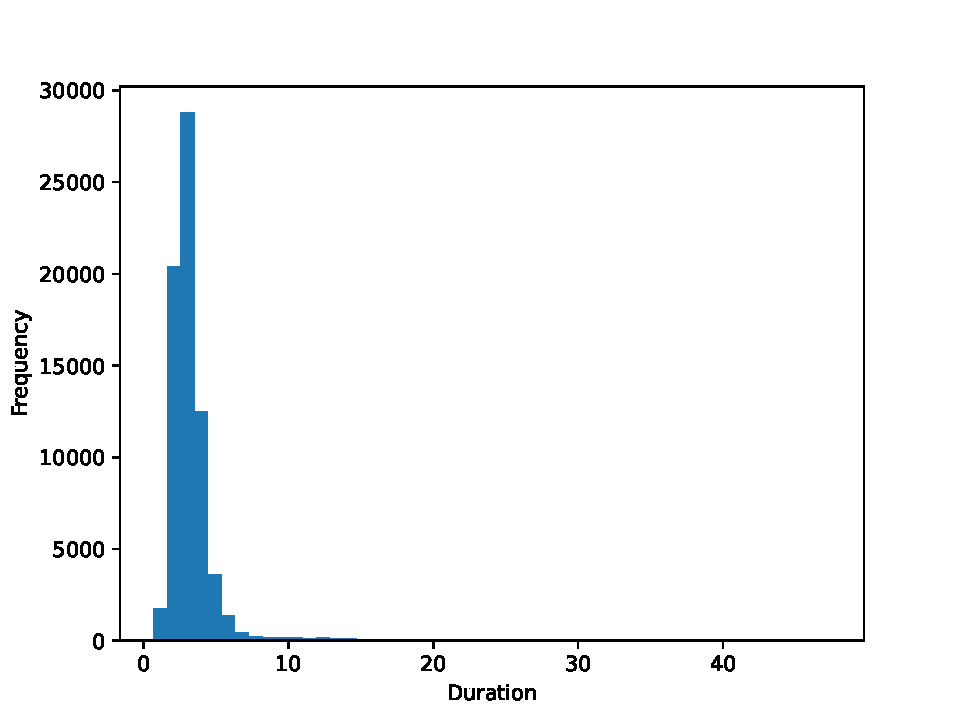
\includegraphics[width=\linewidth]{before_histogram_af.pdf}
    \end{minipage}%
    \begin{minipage}{.50\textwidth}
      \centering
      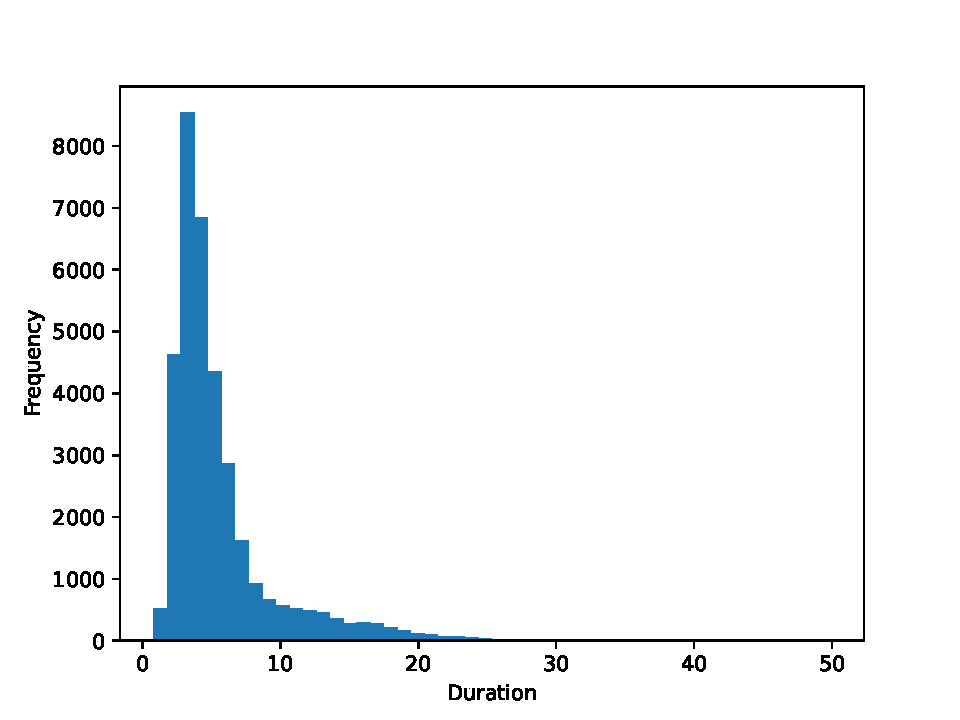
\includegraphics[width=\linewidth]{before_histogram_xh.pdf}
    \end{minipage}
    \caption{The histograms of the recording durations of the Afrikaans dataset (left) and the isiXhosa dataset (right) \textbf{without removing outliers}.}
    \label{fig:histogram1}
\end{figure}

\begin{figure}[!ht]
    \centering
    \begin{minipage}{.50\textwidth}
      \centering
      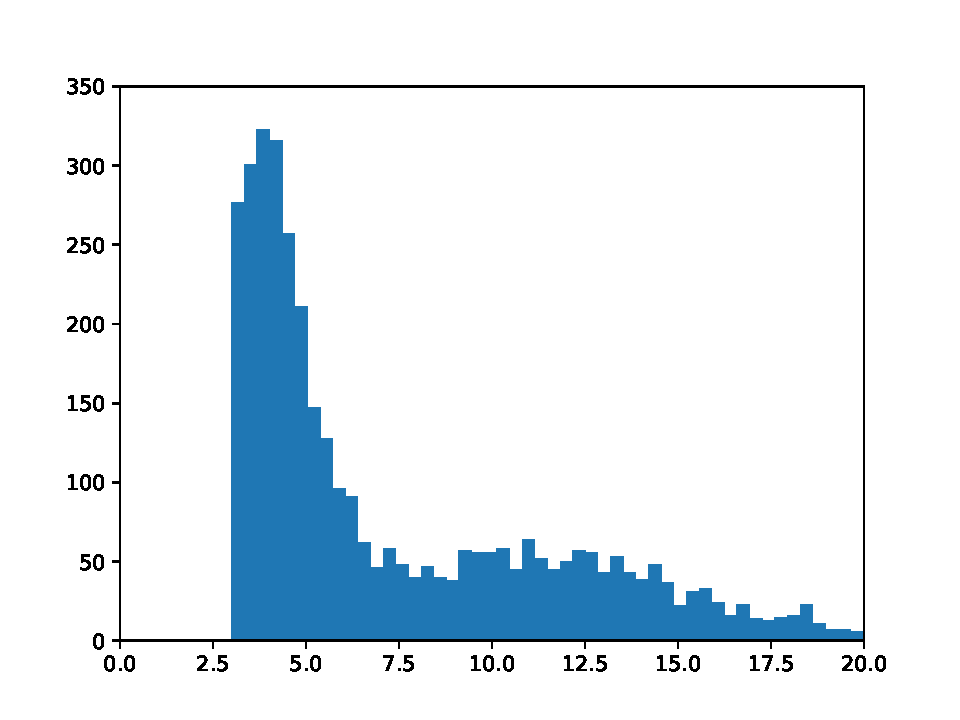
\includegraphics[width=\linewidth]{final_histogram_af.pdf}
    \end{minipage}%
    \begin{minipage}{.50\textwidth}
      \centering
      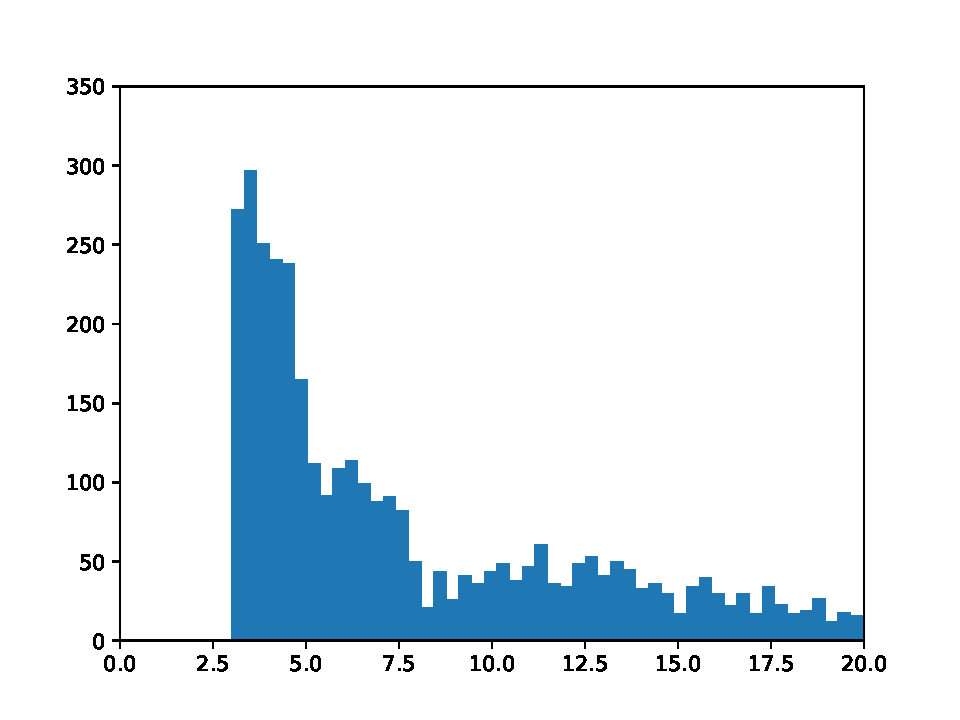
\includegraphics[width=\linewidth]{final_histogram_xh.pdf}
    \end{minipage}
    \caption{The histograms of the recording durations of the Afrikaans dataset (left) and the isiXhosa dataset (right) \textbf{after removing outliers}.}
    \label{fig:histogram2}
\end{figure}

Both datasets contain approximately $7.5$ hours of speech recordings (after removing outliers). 
Additionally, we ensure that the validation and test data does not contain recordings of speakers that appear in the training data (\ref{par:excl_split}).
The transcription texts are pre-processed in the same way as the LM data, which is explained in the following section.

\newpage

\subsection{Language model data}
The data used for training the LM (\ref{subsec:lm-boost}) consists of Afrikaans and isiXhosa \href{https://dumps.wikimedia.org/}{Wikipedia dumps}.
The text is extracted from the dumps using a tool called the WikiExtractor \cite{Wikiextractor2015}.
The text is pre-processed by converting all characters to lowercase, removing all characters that are not used in the Afrikaans
and isiXhosa language, and removing punctuation marks and other special characters.

\section{Evaluation metric}

\paragraph*{Word error rate} \label{subsec:wer}
The word error rate (WER) \cite{WordErrorRate} is equal to the number of character-level errors in the predicted transcript, 
divided by the number of words in the true transcript. One character-level error is corrected using one of three operations:
inserting a new character, deleting an existing character, or substituting an existing character for a new character.
\\
\\
That concludes our experimental setup. Firstly, we discussed our main research question and how we will attempt to solve it using different experiments.
Secondly, we explained our approach for collecting Afrikaans, Dutch, isiXhosa, and isiZulu speech data.
Finally, we briefly discussed the training data for our LM, and we briefly explained the WER metric.